\begin{surferPage}[Cayley-flaten]{Cayley-flaten av tredje grad}
Denne flaten av tredje grad har fire singulariteter. Den har fått navn etter Arthur Cayley, som forsket mye på slike flater på 1800-tallet.
    
    Det var imidlertid Ludwig Schlãfli som først klassifiserte disse flatene i 1863. Han systematiserte dem etter hvilke typer singulariteter flatene kunne ha.
	For eksempel kan man i artikkelen hans lese om hvorfor det ikke kan være mer enn $4$ singulære punkter på en flate av tredje grad
    det vil si at: $\mu(3)=4$. 
    
Rundt 1900 studerte Felix Klein de mulige formene til reelle flater av tredje grad. Hans løsning var å starte med Cayley-flaten av tredje grad og legge små deformasjoner til denne: Ved å trekke fra hverandre eller føre sammen de doble kjeglene, kunne han finne alle de mulige formene som flater av tredje grad kan ha. Her er noen av dem: 
    \vspace{0.3cm}
     \begin{center}
      \vspace{-0.2cm}
      \begin{tabular}{@{}c@{\ }c@{\ }c@{\ }c@{}}
        \begin{tabular}{@{}c@{}}
          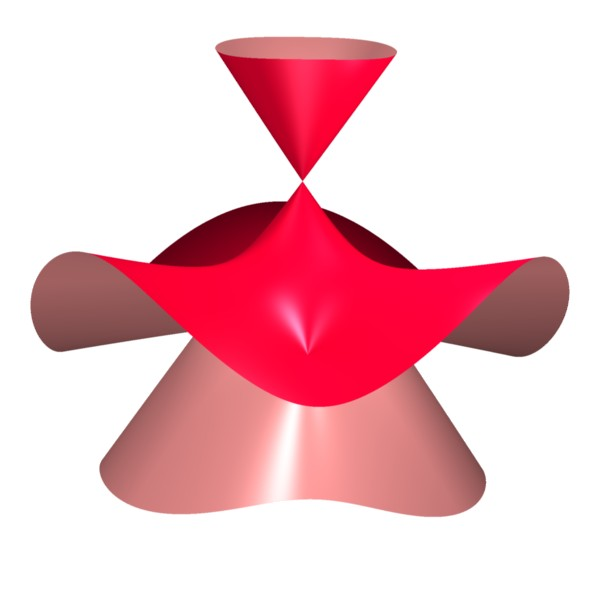
\includegraphics[width=1.35cm]{./../../common/images/cayley_cubic_0}
        \end{tabular}
        &
        \begin{tabular}{@{}c@{}}
          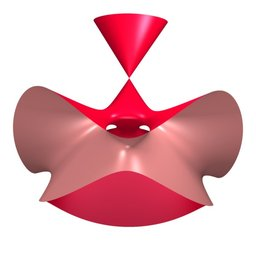
\includegraphics[width=1.35cm]{./../../common/images/cayley_cubic_1}
        \end{tabular}
        &
        \begin{tabular}{@{}c@{}}
          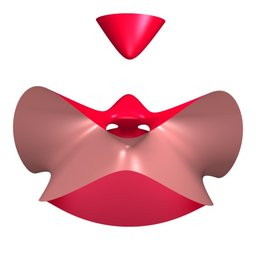
\includegraphics[width=1.35cm]{./../../common/images/cayley_cubic_2}
        \end{tabular}
        &
        \begin{tabular}{@{}c@{}}
          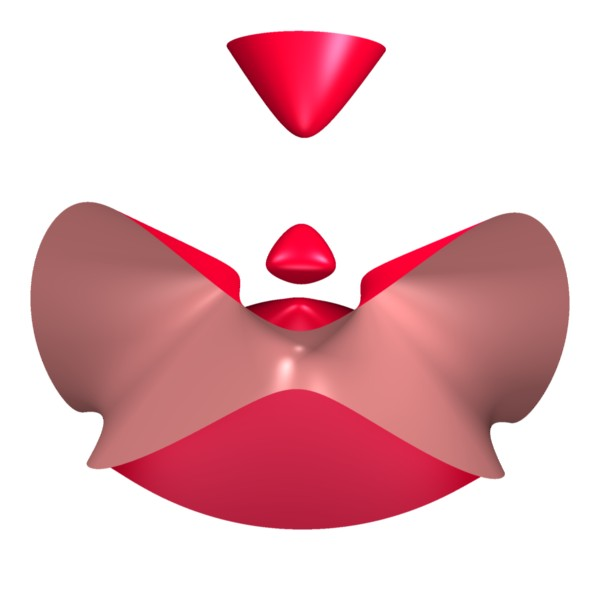
\includegraphics[width=1.35cm]{./../../common/images/cayley_cubic_3}
        \end{tabular}
      \end{tabular}
    \end{center}
\end{surferPage}
